
\section{Глава 4. Создание экспериментального образца}

\subsection{Сборка квадрокоптера}
На основе компонентов, указанных в главе "Разработка архитектуры микродрона" собирается квадрокоптер. На раму устанавливаются все обозначенные компоненты. Фазы каждого мотора припаиваются на соответствующие площадки регуляторов. При проверке вращения моторов в случае несоответствия вращения мотора схеме для px4, необходимо перепаять любые две фазы этого мотора. Также к регуляторам припаиваются силовые провода с коннектором для подключения аккумулятора. Полетный контроллер располагается на виброизоляционных прокладках и подключается к регуляторам через колодку. Далее производится монтаж FPV оборудования, приемника и телеметрийного модуля (рис. \ref{fig:quad1}).
% ~\ref{fig:quad1}
\begin{figure}[H]
	\centering
	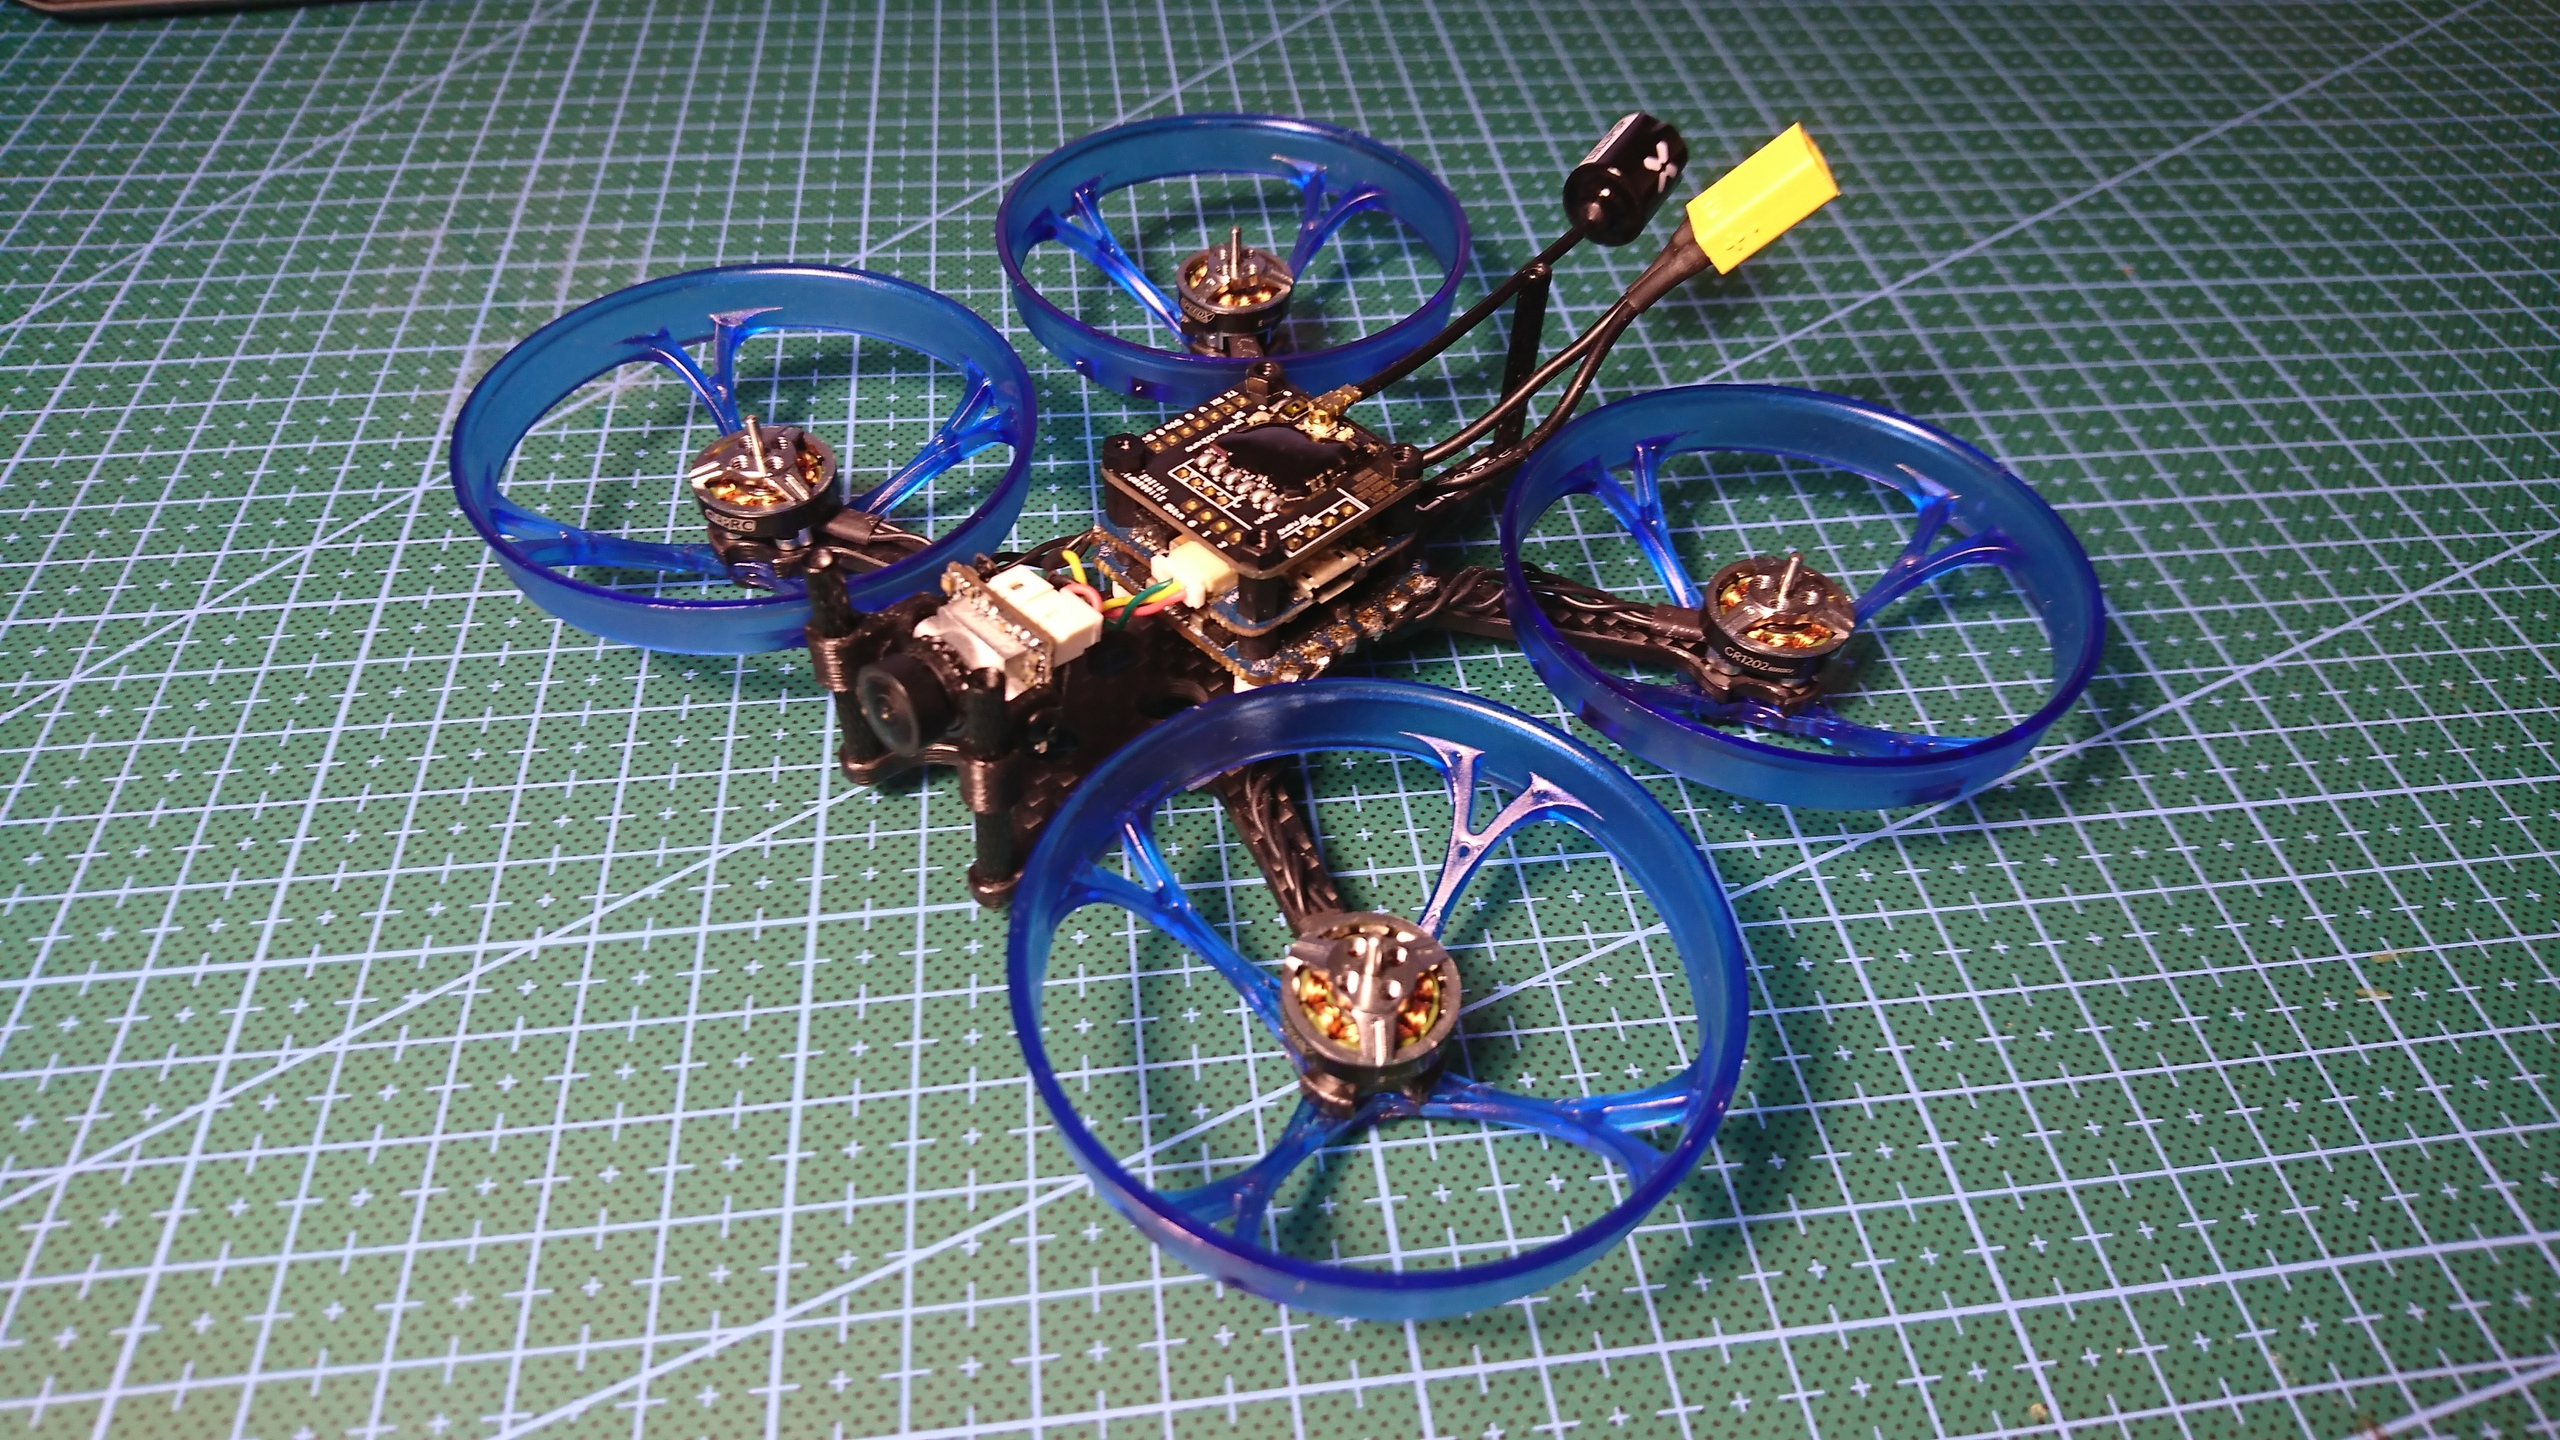
\includegraphics[width=0.5\linewidth]{../RW/pics/quad1}
	\caption{Установка компонентов на раму
	}
	\label{fig:quad1}
\end{figure}
Прикручивается верхняя пластина рамы, закрепляются все свисающие детали и на этом сборка завершается (рис. \ref{fig:quad2}).
% ~\ref{fig:quad2}
\begin{figure}[H]
	\centering
	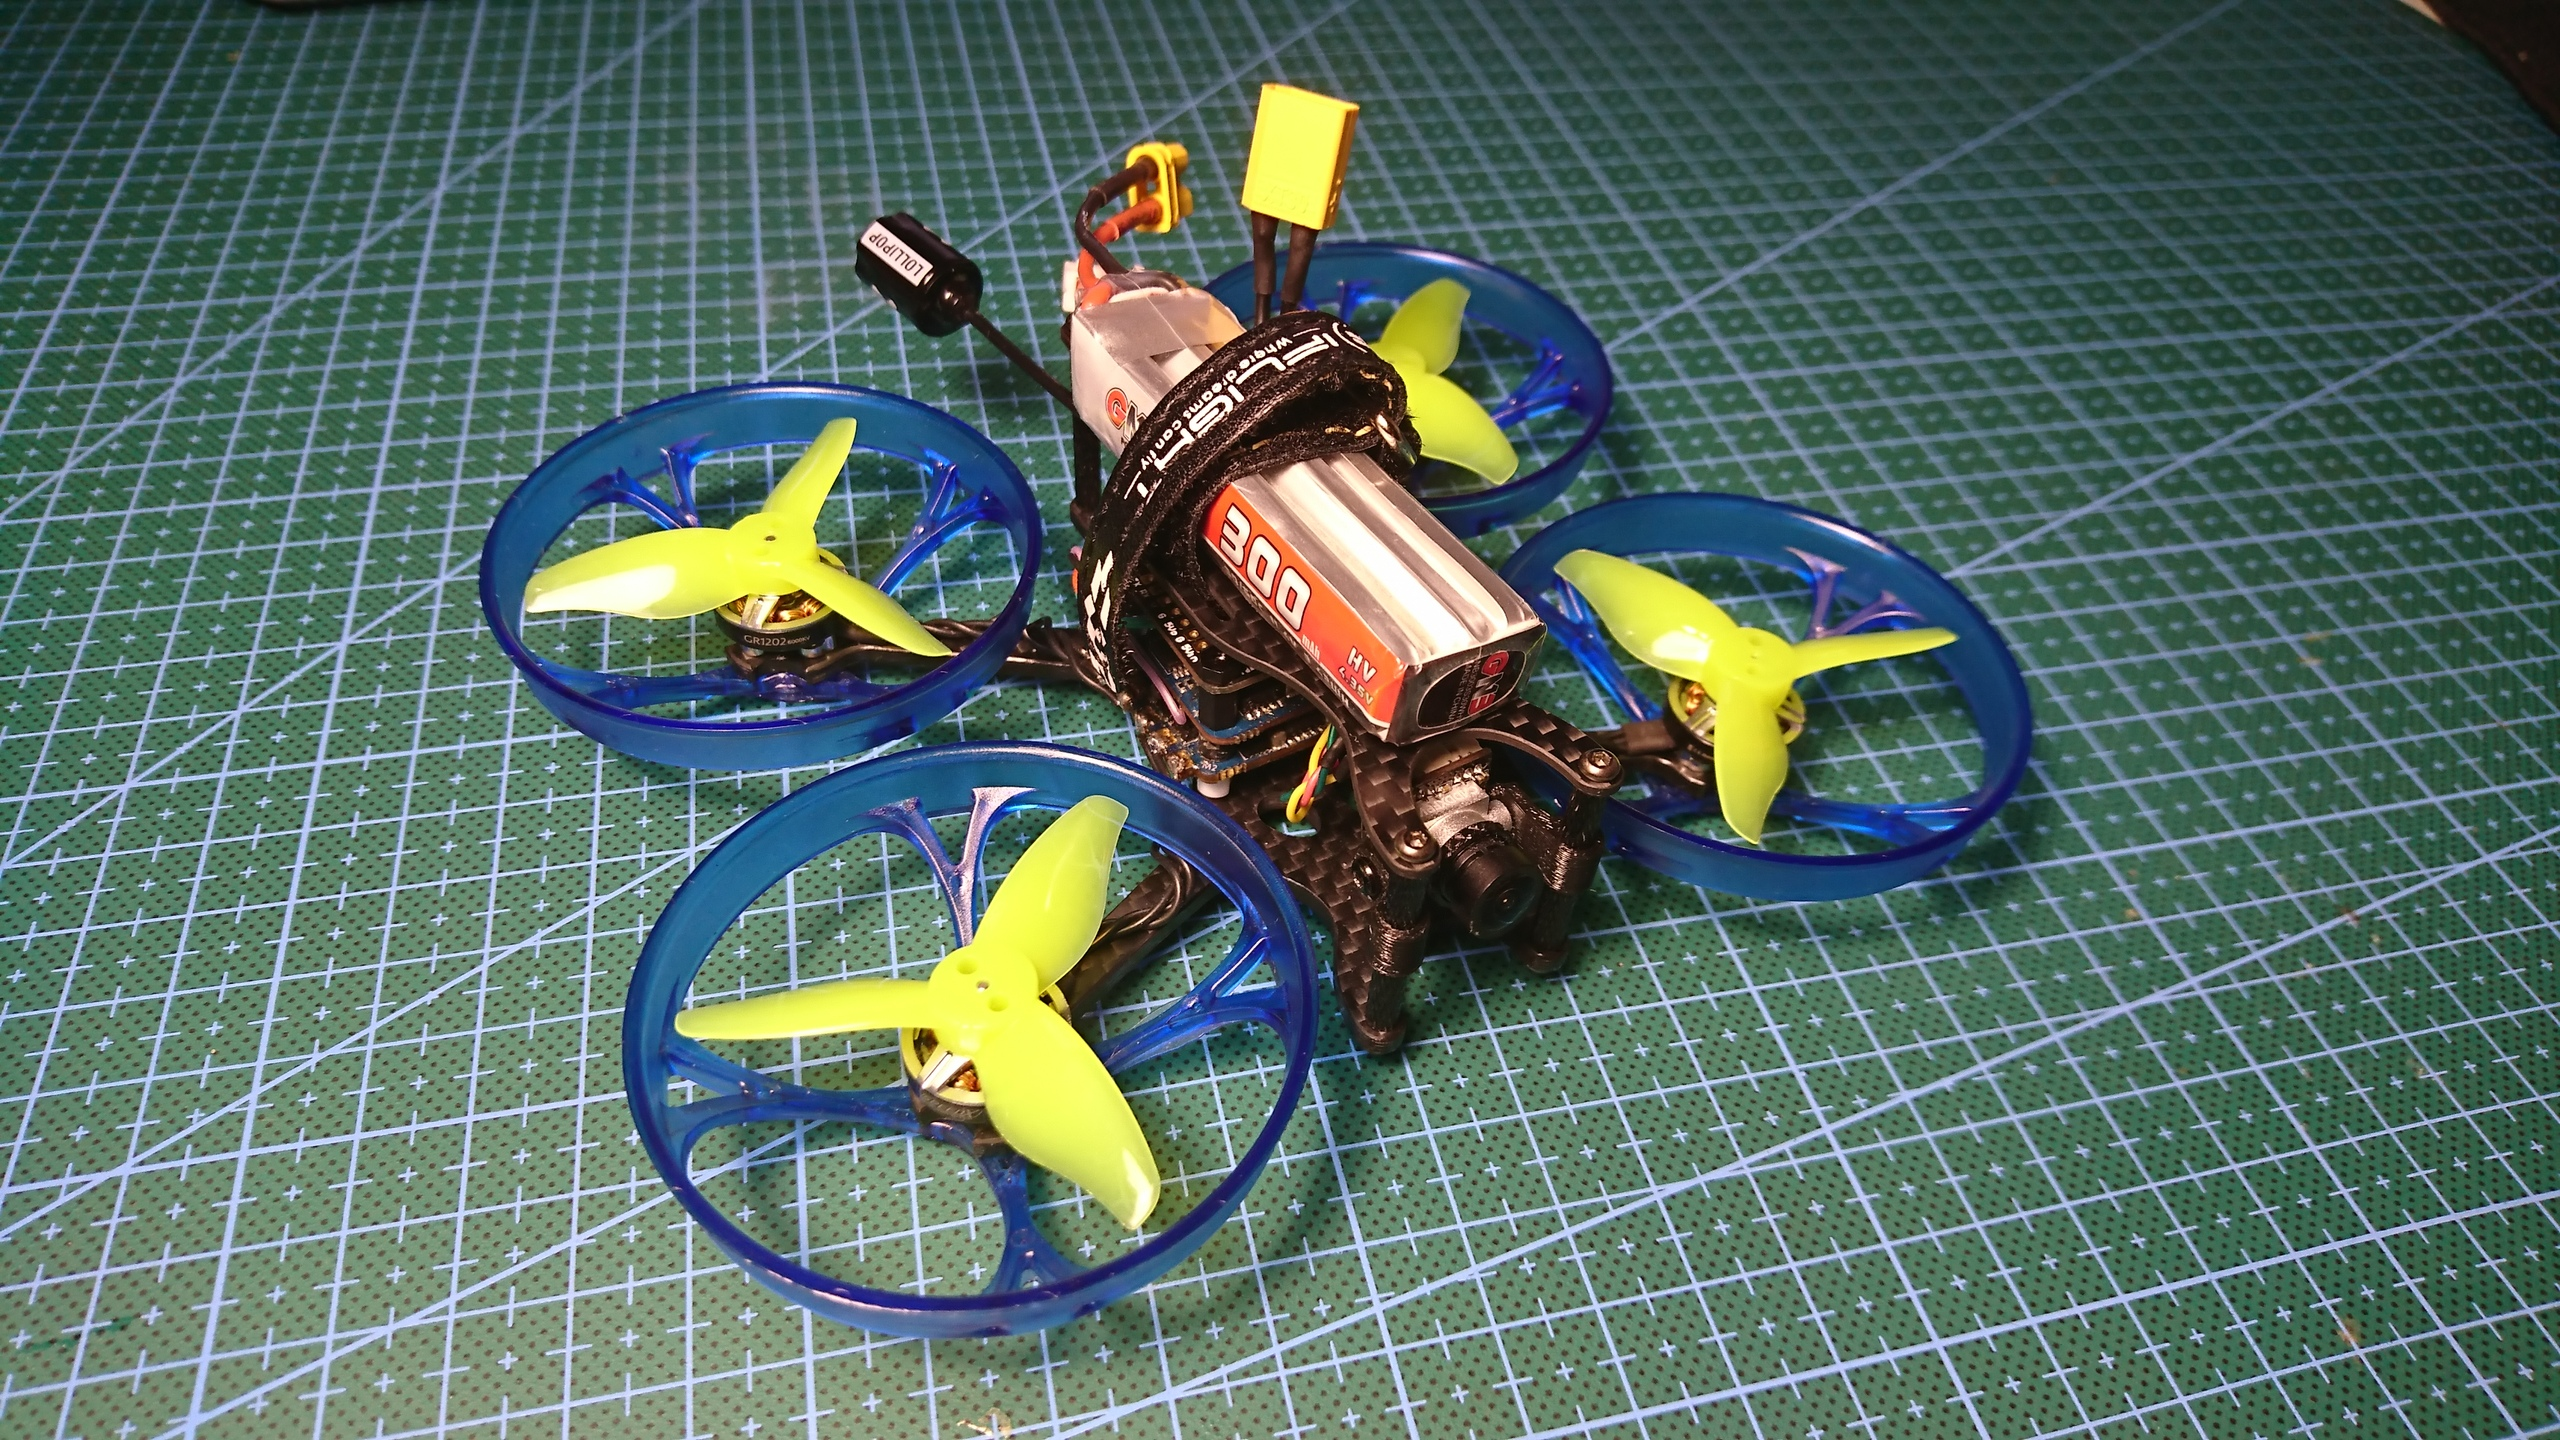
\includegraphics[width=0.5\linewidth]{../RW/pics/quad2}
	\caption{Экспериментальный образец квадрокоптера
	}
	\label{fig:quad2}
\end{figure}

\subsection{Сборка наземной станции}
Согласно шагам из главы "Разработка архитектуры наземной станции" про\-из\-водится подключение всех компонентов наземной станции.
\subsection{Обновление и настройка параметров ПО}
На полетный контроллер через qgroundcontrol по USB прошивается последний образ PX4 из репозитория clover. Производится калибровка всех датчиков. Для взаимодействия приемника с радиомодулем требуется выполнение процедуры привязки -- bind.
Настраиваются бод -- рейты устройств приема-передачи телеметрии на максимально доступное значение. Для экспериментального образца использовались устройства 3DR с бод -- рейтами 115200. При подключении через 3DR модули параметры квадрокоптера считались и отобразились в конфигураторе. Остается настройка базовой станции. Видеоприемник настраивается на диапазон частот видеопередатчика в режиме автопоиска сигнала. Окружение для наземной станции создавалось на базе пакета clover, где предустановлены все необходимые инструменты. В launch файлах меняются параметры для способа подключения, чтобы была доступна симуляция окружения квадрокоптера. Для топика указывается порт, к которому подключен видеомодуль. После перезагрузки применяются параметры и можно приступать к тестированию.
\subsection{Проверка работы экспериментального образца}
Для проверки работы aruco\_detect создается карта маркеров, прописанная в конфигурационном файле пакета clover (рис. \ref{fig:map}).
% ~\ref{fig:map}
\begin{figure}[H]
	\centering
	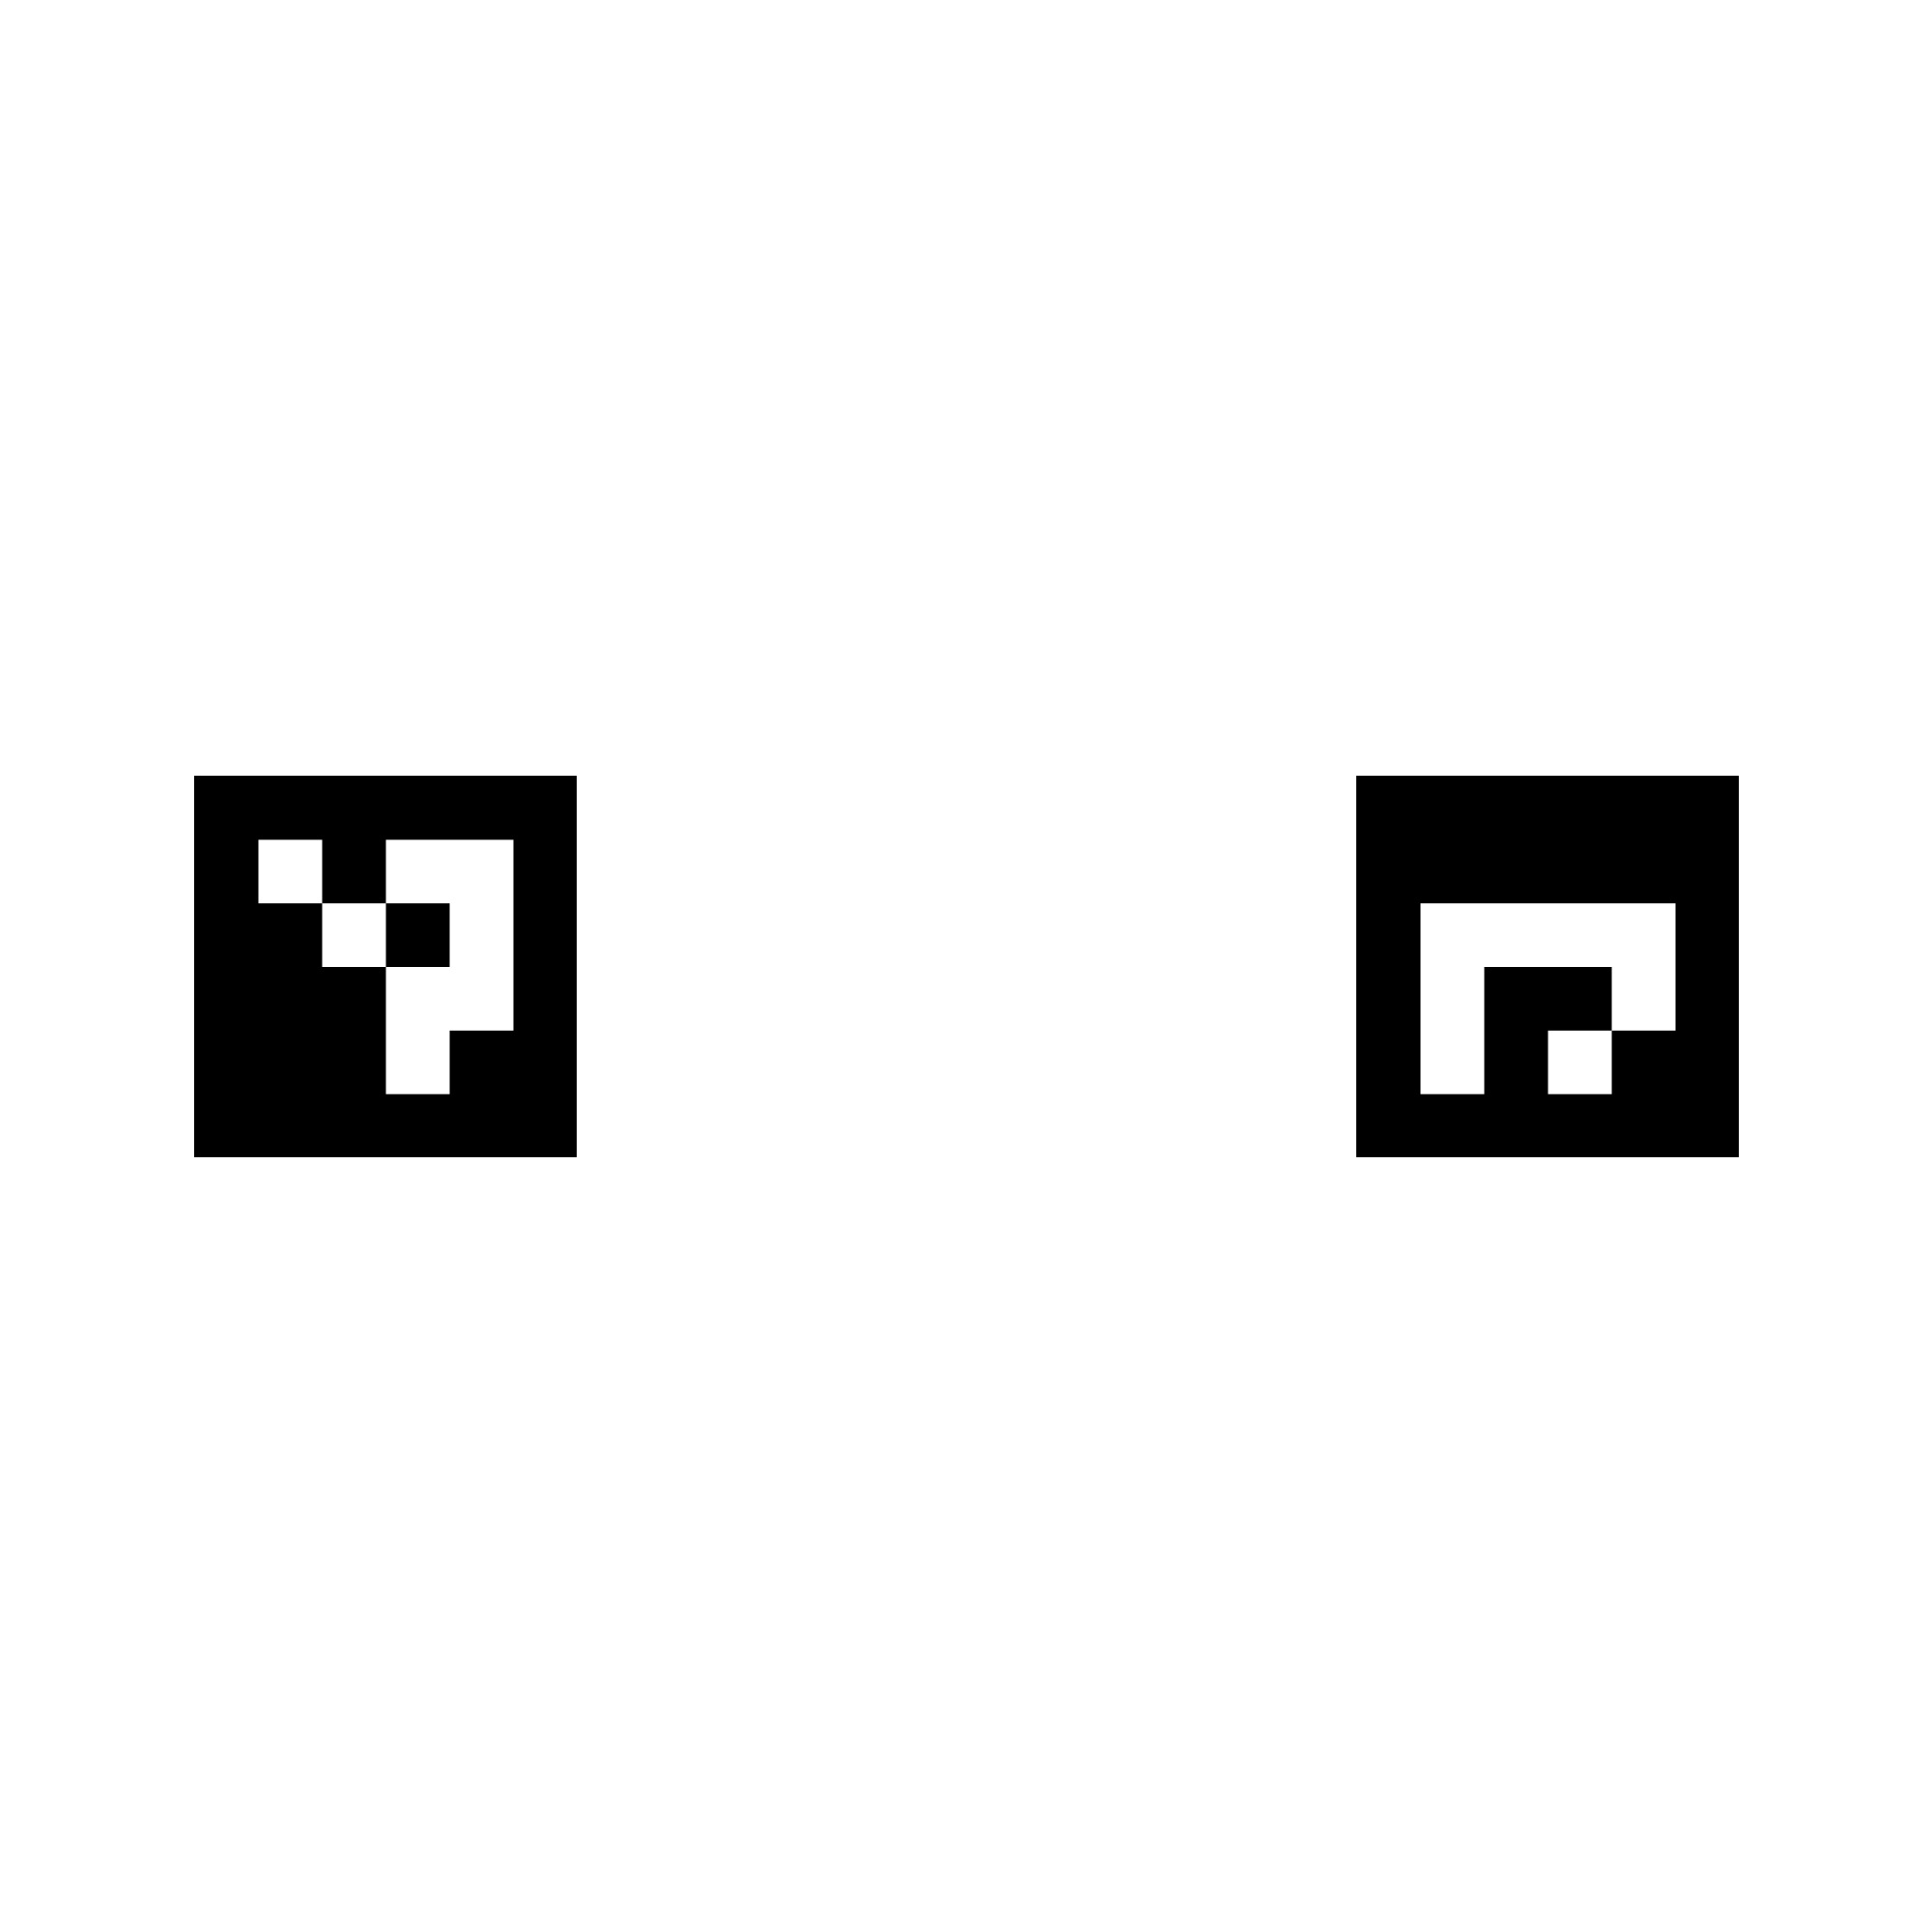
\includegraphics[width=0.5\linewidth]{../RW/pics/map}
	\caption{Карта маркеров
	}
	\label{fig:map}
\end{figure}
Наводим камеру квадрокоптера на метки, проверяем топик aruco\_detect и получаем идентификаторы ме